Consider the following Petri net:



\begin{centering}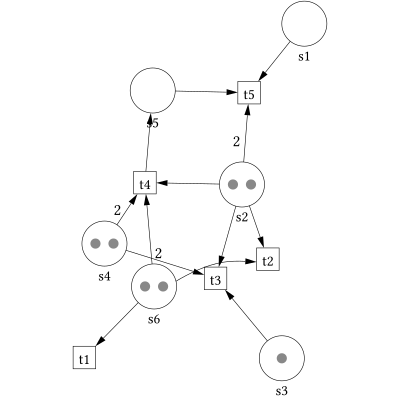
\includegraphics[min width=0.4\textwidth=0.6\textwidth,min height=0.4\textwidth=0.6\textwidth,keepaspectratio,max width=0.9\textwidth,max height=0.9\textwidth]{64/conflictpetri03bbf21bcfa3adcc48836073b75bc6576d6c0f9a2f6acd3b1d10d82bb6fa480211011.pdf}\end{centering}

Which pair of transitions is in conflict, and because of which conflict-causing place(s), under the initial marking?

State your answer by giving a pair of conflicting transitions and a list of all the places that induce the conflict. Stating \begin{verbatim}((t0,t1),[s0,s1])\end{verbatim} as answer would indicate that transitions t0 and t1 are in conflict under the initial marking
and that places s0 and s1 are all those common places within the preconditions
which each separately do not have enough tokens for firing t0 and t1 at the same time. The order of transitions within the firstly given pair does not matter here.
The order of places within the listing of places inducing the conflict is irrelevant as well.

Please note: When hovering over or clicking on edges / nodes or their labels, the respective components that belong together are highlighted.

